% Structure of the Riemann solution for variable-coefficient nonlinear elasticity (chapter
% Nonlinear_elasticity): a left-going wave, the stationary wave at x = 0 and a right-going
% wave. Make the SVG with figures/src/build.sh.
\documentclass[12pt, border=0pt]{standalone}
% Shared style of the Riemann-structure diagrams (shallow_water_riemann.tex,
% nonlinear_elasticity_riemann.tex): waves in the x-t plane and the constant states.
\usepackage{amsmath}
\usepackage{tikz}
\usetikzlibrary{backgrounds}
\definecolor{state}{RGB}{31,78,156}
\tikzset{
  every picture/.style={line cap=round, show background rectangle,
                        background rectangle/.style={fill=white}, inner frame sep=6pt},
  axis/.style={line width=0.9pt},
  wave/.style={line width=0.9pt},
  fan/.style={line width=0.35pt},
  stationary/.style={line width=0.9pt, dash pattern=on 4pt off 3pt},
  state/.style={text=state},
}
% A rarefaction fan from the origin: edge speeds #1 and #2 (dx per unit height), height #3
\newcommand{\fan}[3]{%
  \foreach \k in {1,2,3} {\draw[fan] (0,0) -- ({(#1 + \k*(#2-#1)/4)*#3}, #3);}
  \draw[wave] (0,0) -- ({#1*#3}, #3);
  \draw[wave] (0,0) -- ({#2*#3}, #3);}
% A state vector with entries #1 and #2
\newcommand{\state}[2]{$\begin{bmatrix} #1 \\ #2 \end{bmatrix}$}

\begin{document}
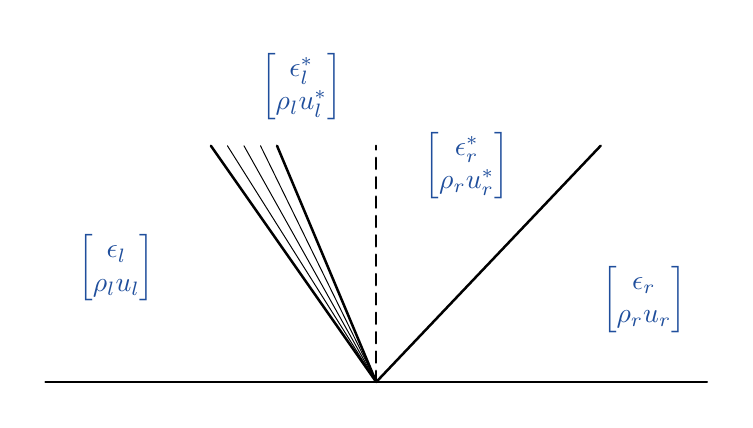
\begin{tikzpicture}
  \draw[axis] (-4.2,0) -- (4.2,0);
  \fan{-0.7}{-0.42}{3}
  \draw[stationary] (0,0) -- (0,3);
  \draw[wave] (0,0) -- (2.85,3);
  \node[state] at (-3.3,1.45) {\state{\epsilon_l}{\rho_l u_l}};
  \node[state] at (-0.95,3.75) {\state{\epsilon_l^*}{\rho_l u_l^*}};
  \node[state] at (1.15,2.75) {\state{\epsilon_r^*}{\rho_r u_r^*}};
  \node[state] at (3.4,1.05) {\state{\epsilon_r}{\rho_r u_r}};
\end{tikzpicture}
\end{document}
